\documentclass{article}
\usepackage{arxiv}

\usepackage[utf8]{inputenc}
\usepackage[english, russian]{babel}
\usepackage[T1]{fontenc}
\usepackage{url}
\usepackage{booktabs}
\usepackage{amsfonts}
\usepackage{nicefrac}
\usepackage{microtype}
\usepackage{lipsum}
\usepackage{graphicx}
\usepackage{natbib}
\usepackage{doi}



\title{Метод построения случайного леса на основе отдаления друг от друга базовых моделей}

\author{ Дмитриев Леонид Алексеевич  \\
	МГУ им. М.В. Ломоносова\\
	ф-т ВМК, кафедра ММП\\
	% Pittsburgh, PA 15213 \\
	\texttt{s02200542@gse.cs.msu.ru} \\
	%% examples of more authors
	\And
	д.ф-м.н. Сенько Олег Валентинович \\
	МГУ им. М.В. Ломоносова\\
	ф-т ВМК, кафедра ММП\\
	% Santa Narimana, Levand \\
	\texttt{senkoov@mail.ru } \\
	%% \AND
	%% Coauthor \\
	%% Affiliation \\
	%% Address \\
	%% \texttt{email} \\
	%% \And
	%% Coauthor \\
	%% Affiliation \\
	%% Address \\
	%% \texttt{email} \\
	%% \And
	%% Coauthor \\
	%% Affiliation \\
	%% Address \\
	%% \texttt{email} \\
}
\date{}

\renewcommand{\shorttitle}{Метод случайного леса}


\begin{document}
\maketitle

\begin{abstract}
	В работе представлен новый метод случайного леса, который строится итеративно и в котором новое дерево обучается с учетом накопленного до него ансамбля. Данный метод хорошо проявляет себя на некоторых химических и медицинских данных. Исследование метода проводилось на датасете кристаллических решеток.
\end{abstract}


\keywords{Machine Learning \and Multilevel Machine Learning Systems \and Regression Modeling \and Inorganic Compounds Physical Properties Prediction.}

\section{Введение}

Случайный лес - широко известный алгоритм машинного обучения.
Его способность хорошо аппроксимировать данные за счёт
уменьшения разброса основана на предположении, что все деревья
ансамбля независимы и различны. Но практическое уменьшение
разброса значительно меньше теоретического, так как на деле
получаемые деревья обучаются на объектах из одного и того же
множества. Это проблема частично решается такими методами, как
беггинг и бутстрап.
Предлагается другой способ повышения разнообразия деревьев
внутри леса. Вместо независимой и параллельной генерации деревьев,
будем на каждом шагу добавлять дерево, сильно отличающееся от уже
созданного ансамбля, с помощью специального функционала,
учитывающего ответы предыдущих моделей. Выдвигается гипотеза,
что данный метод повысит разнообразие деревьев в ансамбле и тем
самым уменьшит разброс предсказаний.
Помимо отличия от предыдущих моделей, следующему дереву можно
придать свойства какого-либо другого метода, например градиентного
бустинга. Это может сделать лес не только разнообразным, но и более
качественным.
В данной работе будет детально рассмотрено построение дерева на
очередном шаге по вышеописанному методу и для тестирования будет
исследовано его применение на данных о химических веществах.
\citep{bibref1}, \citep{bibref2}, \citep{Ren_2015_CVPR}, \citep{bibrel3}.

\section{Постановка задачи}
\label{sec:headings}

\section{Теория}

Предположим, что у нас есть переменная $Y$, стохастически зависящая от вектора переменных $X_1, \dots, X_n$, 
функции $G_1(x)$, $G_2(x)$, детерминировано зависящие от вектора переменных $X_1, \dots, X_n$.

Имеется выборка $\tilde{S} = \{ (y_j, x_j, G_1(x_j), G_2(x_j)), j = \overline{1, m} \}$, где
\begin{itemize}
	\item $y_j$ - значение переменной $Y$ для объекта с номером $j$
	\item $x_j = (x_{j1}, \dots, x_{jn})$ - вектор значений признаков $X_1, \dots, X_n$ для объекта с номером $j$
	\item $G_1(x_j)$ - значение функции $G_1$ в точке $x_j$
	\item $G_2(x_j)$ - значение функции $G_2$ в точке $x_j$
\end{itemize}

Предлагается построить дерево $T(x)$, для которого достигается минимум функционала:
$$ \Phi(\tilde{S}, T) = \Sigma_{j=1}^{m} \{ \gamma_1 [T(x_j) - y_j]^2 + \gamma_2 [T(x_j) - G_2(x_j)]^2 - \mu [T(x_j) - G_1(x_j)]^2   \}  $$
где $\gamma_1 + \gamma_2 = 1; \quad \gamma_1, \gamma_2, \mu \in [0, 1] $


Как видно из структуры функционала $\Phi$, дерево $T$, соответствующее его минимуму,  будет аппроксимировать связь $Y$ с переменными $X_1, \dots, X_n$ при $\gamma_1 > 0$.

Одновременно дерево $T(x)$ будет удаляться от зависимости $G_2(x)$ при возрастании $\mu$ и приближаться к зависимости $G_1(x)$ при возрастании $\gamma_2$.


\subsection{Реализация дерева}

При построении дерева был использован "жадный" \space метод оптимизации целевого функционала: на каждом шагу к дереву добавляется узел, обеспечивающий наибольшее снижение используемого функционала $\Phi$.

Предположим, что на каком-то шаге дерево $T_k$ содержит $k$ концевых узлов, которым соответствуют концевые выборки $S_1^k, \dots, S_k^k$.

Новое дерево $T_{k + 1}$ строится через добавление к дереву $T_k$ дополнительного узла $u$.

Узел $u$ получается из некоторого концевого узла $g$ с помощью порогового правила вида $X_u > \delta_u$, где $X_u$ и $\delta_u$ признак и порог к нему соответственно. 

Правило $X_u > \delta_u$ расщепляет выборку $S_g^k$ на две подвыборки.

Признак $X_u$ и порог $\delta_u$ ищутся из условия максимизации разности $\Phi(\tilde{S}, T_k) - \Phi(\tilde{S}, T_{k + 1})$.

Процесс построения может быть прекращен при выполнении одного из перечисленных условий:

\begin{itemize}
	\item На очередном шаге не удается уменьшить функционал
	\item На очередном шаге произошло изменение функционала, меньшее чем некоторое пороговое значение
	\item Кол-во объектов внутри узла меньше некоторого порогового значения
\end{itemize}




\section{Эксперименты}

\subsection{Описание данных}

Для тестирования реализации дерева было использовано два набора данных с разным множеством признаков. Данные состоят из двух разных датасетов химических соединений.

Объектами являются некоторые химические соединения, каждый из которых описан набором вещественных значений. Целевой переменной является температура плавление химического соединения в Кельвинах.

Проведем некоторый анализ предоставленных данных. Первый датасет имеет 451 объект и 98 признаков, а второй 431 объект и 86 признаков. Данные были разделены на тренировочную и тестовую выборки в соотношении 7 к 3.

\begin{figure}[h]
	\begin{center}
		\begin{minipage}[h]{0.95\linewidth}
			{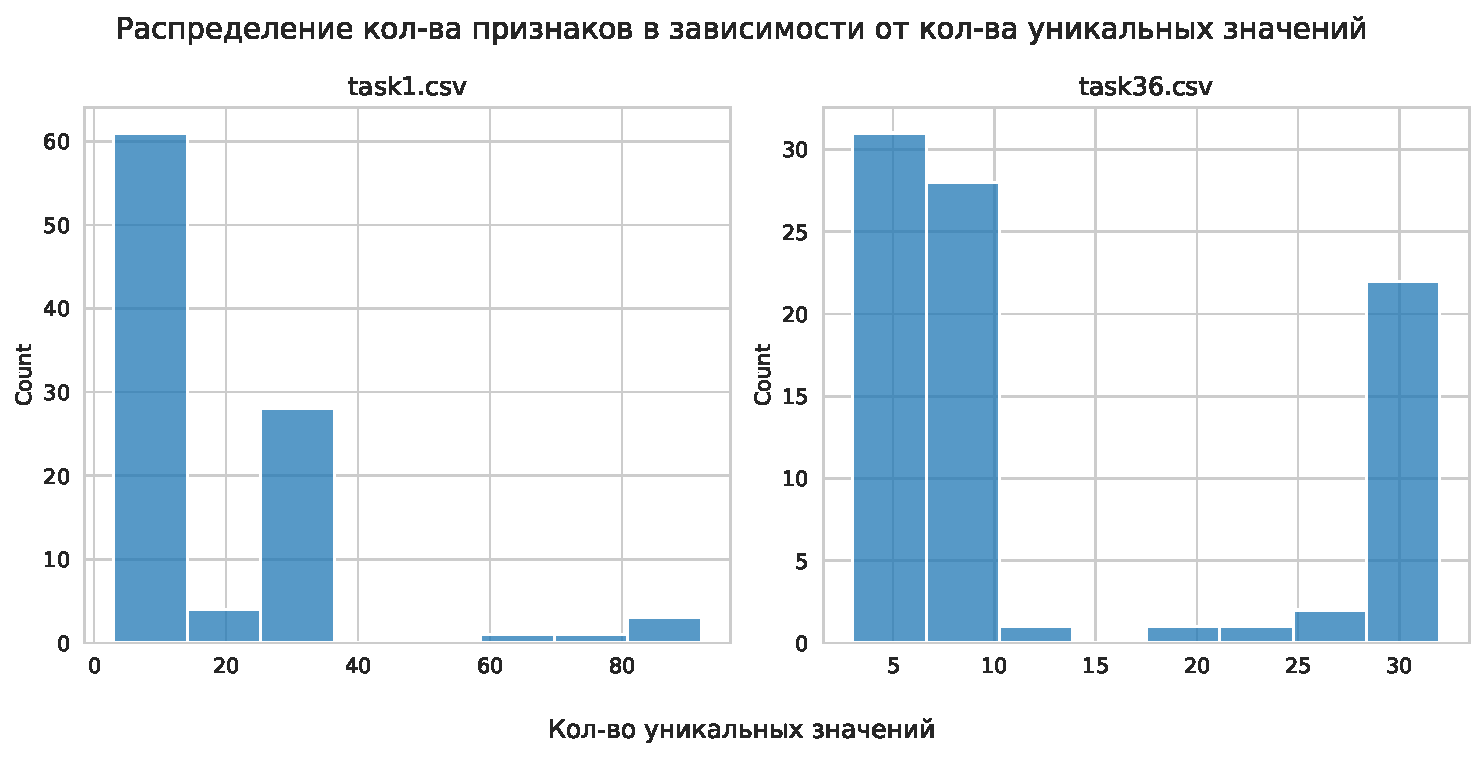
\includegraphics[width=1.0\linewidth]{../figures/dists.pdf}}	
		\end{minipage}
	\end{center}
	
	\caption{График распределения кол-ва признаков в зависимости от кол-ва уникальных значений. }
	
	\label{ris:image1}
	
\end{figure}

Из данных графиков на рис. \ref{ris:image1} можно заметить, что у большей части признаков в датасете малое число уникальных значений. Из этого можно сделать вывод, что признаки можно интерпретировать как упорядоченные категориальные, как раз для таких данных хорошо подходит модель решающего дерева.


\begin{figure}[h]
	\centering
	
	\begin{minipage}[h]{\linewidth}
		{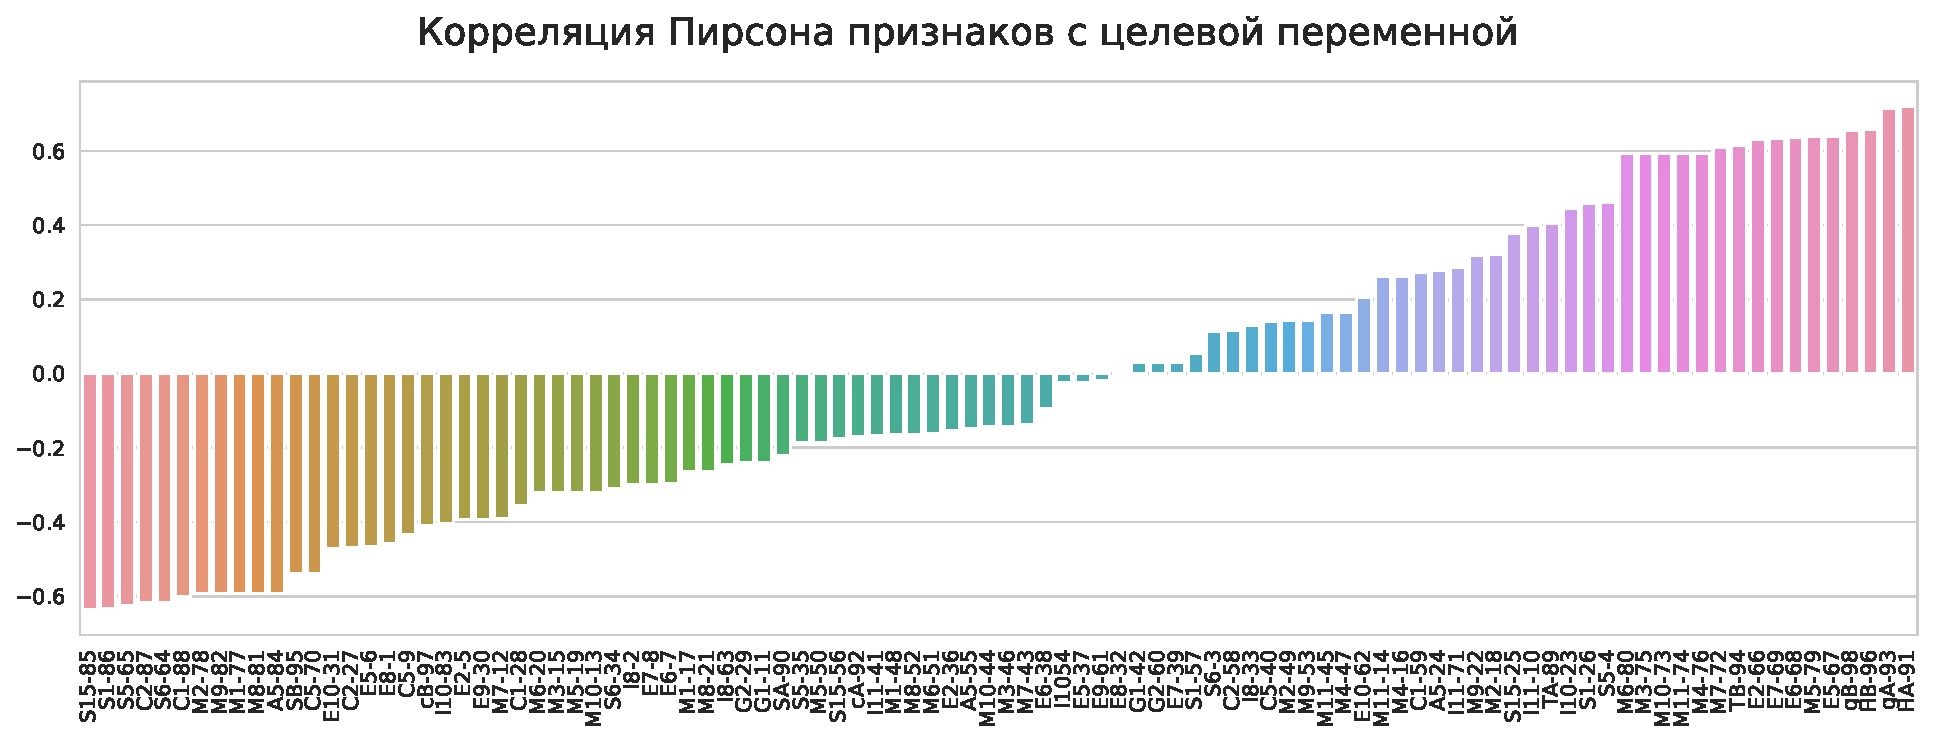
\includegraphics[width=1.0\linewidth]{../figures/corr_task1.pdf}}	
	\end{minipage}
	
	\caption{График корреляции Пирсона признаков с целевой переменной из датасета 1 }
	\label{ris:image2}
\end{figure}

\begin{figure}[h]
	\centering
	
	\begin{minipage}[h]{\linewidth}
		{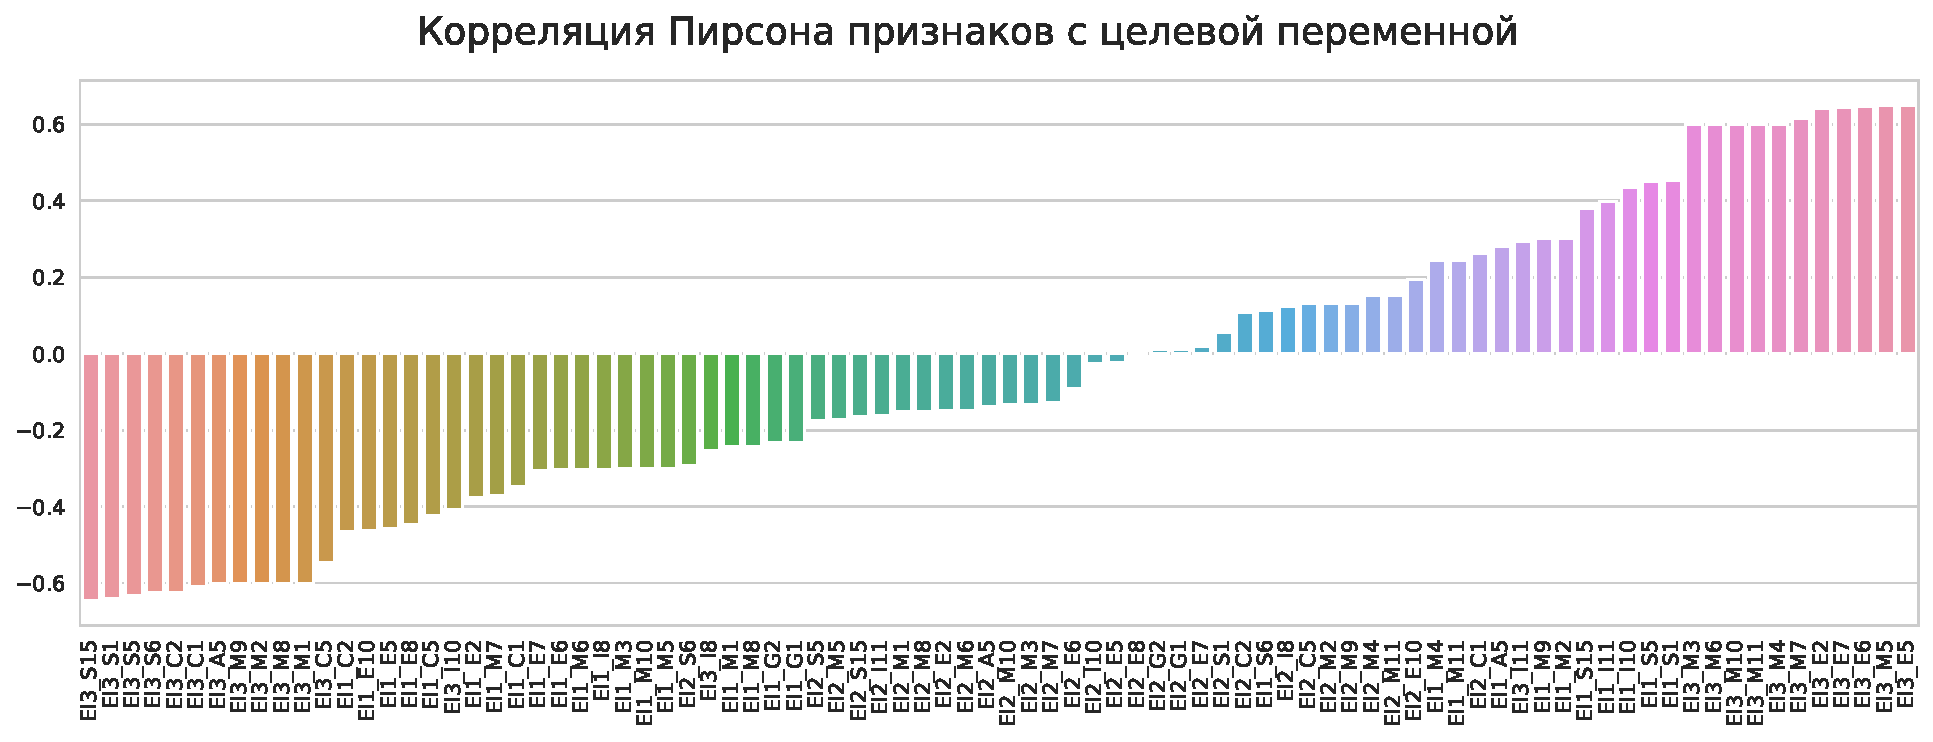
\includegraphics[width=1.0\linewidth]{../figures/corr_task36.pdf}}	
	\end{minipage}
	
	
	\caption{График корреляции Пирсона признаков с целевой переменной из датасета task36.csv }
	\label{ris:image3}
\end{figure}

На рис. \ref{ris:image2} и рис. \ref{ris:image3} изображена степень корреляции каждого из признаков с целевой переменной в порядке возрастания. Из данных графиков можно сделать вывод, что признаки имеют высокую степень корреляции с целевой переменной и не являются случайными. К тому же можно заметить, что графики для двух датасетов имеют большое сходство между собой, а значит данные принадлежат одному распределению. Дальнейшее исследование проведем над одним из датасетов.



\subsection{Результаты экспериментов}

Были проведены эксперименты над реализацией дерева решений для задачи регрессии, оптимизирующего рассматриваемый функционал.

Для тестирования и исследования в качестве модели G1 (к зависимости которой дерево должно приближаться) был взят градиентный бустинг, а в качестве модели G2 (от зависимости которой необходимо удаляться) случайный лес. Параметры данных моделей были подобраны на кросс-валидации, где использовалась стандартная метрика MSE.

Был произведен ряд экспериментов с различными значениями гиперпараметров модели, такими как максимальная глубина дерева, минимальное число объектов в узле для разбиения, а также перебирались разные значения параметров целевого функционала: $\gamma_1, \gamma_2, \mu$.

На рис. \ref{ris:image4} и рис. \ref{ris:image5} изображено поведение рассматриваемого функционала в зависимости от глубины дерева. На первом графике в целевом функционале преобладают истинные значения таргета, а на втором преобладают значения, предсказанные градиентным бустингом. 


\begin{figure}[h]
	\begin{center}
		\begin{minipage}[h]{0.95\linewidth}
			{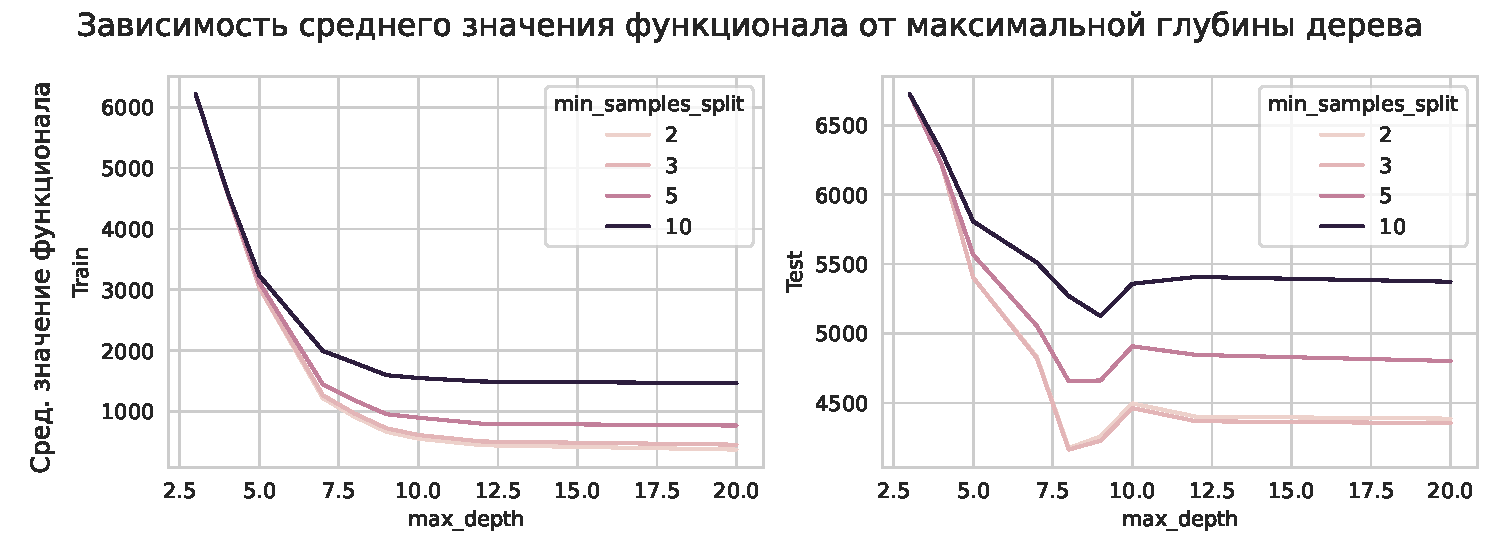
\includegraphics[width=1.0\linewidth]{../figures/max_depth_task1_gamma_08_mu_02.pdf}}	
		\end{minipage}
	\end{center}
	
	\caption{График зависимости значения функционала от глубины дерева для датасета 1 при разных значениях параметра $min\_samples\_split$, и при $\gamma_1 = 0.8$, $\gamma_2 = 0.2$, $\mu = 0.2$. }
	\label{ris:image4}
\end{figure}


\begin{figure}[h]
	\begin{center}
		\begin{minipage}[h]{0.95\linewidth}
			{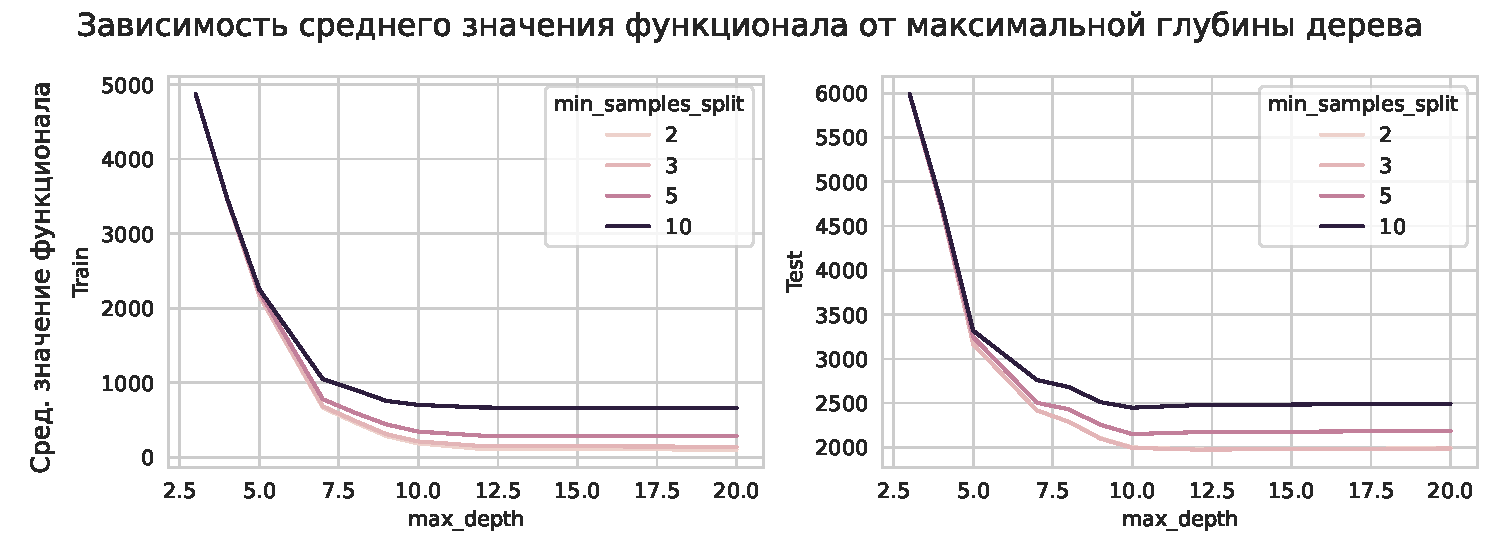
\includegraphics[width=1.0\linewidth]{../figures/max_depth_task1_gamma_02_mu_02.pdf}}	
		\end{minipage}
	\end{center}
	
	\caption{График зависимости значения функционала от глубины дерева для датасета 1 при разных значениях параметра $min\_samples\_split$, и при $\gamma_1 = 0.2$, $\gamma_2 = 0.8$, $\mu = 0.2$. }
	\label{ris:image5}
\end{figure}


На рис. \ref{ris:image4} наблюдается уменьшение значения функционала при уменьшении гиперпараметра $min\_samples\_split$ на тренировочной и тестовой выборках с последующим установлением плато, что связано с достижением предельного значения глубины, после которого во всех узлах минимальное число объектов. При глубине дерева 8 заметен локальный минимум на тестовой выборке, после чего функционал существенно не уменьшался.


На рис. \ref{ris:image5}, где в функционале преобладают предсказания градиентного бустинга, можно заметить, что функционал на тестовой выборке убывает монотоннно, как и на тренировочной выборке. Такое поведение может быть, связано с тем, что для решающего дерева предсказывать ответы градиентного бустинга (основанного на деревьях) проще, чем истинную зависимость.



\begin{figure}[h]
	\begin{center}
		\begin{minipage}[h]{1\linewidth}
			{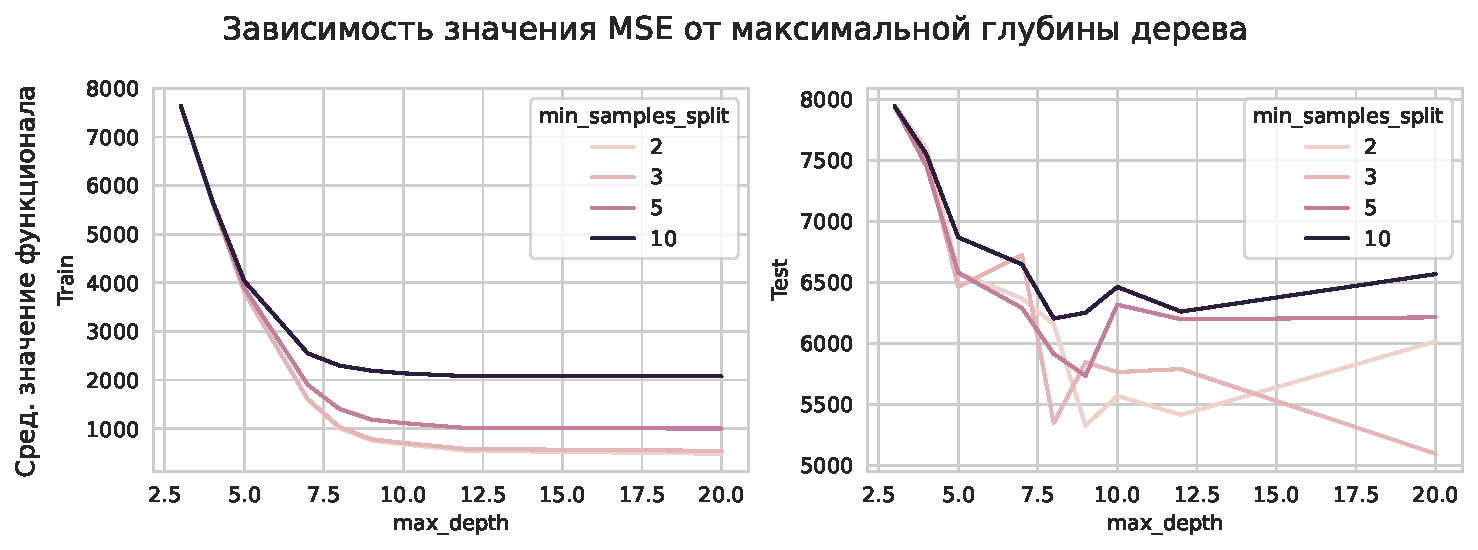
\includegraphics[width=1.0\linewidth]{../figures/task1_common_mse.pdf}}	
		\end{minipage}
	\end{center}
	
	\caption{График зависимости значения MSE от глубины дерева (деревья обучались с метрикой MSE). }
	\label{ris:image6}
\end{figure}

Рассмотрим разницу между поведением исследуемого функционала и стандартного MSE при увеличении максимальной глубины дерева. На рис. \ref{ris:image6} изображен график зависимости метрики MSE от максимальной глубины дерева. На тренировочной выборке MSE монотонно убывает с ростом глубины, что похоже на поведение рассматриваемого функционала, но на тестовой выборке наблюдаются колебания. Можно сделать вывод, что исследуемый функционал оптимизируется стабильнее, чем MSE.


\begin{figure}[h]
	\begin{center}
		\begin{minipage}[h]{1.0\linewidth}
			{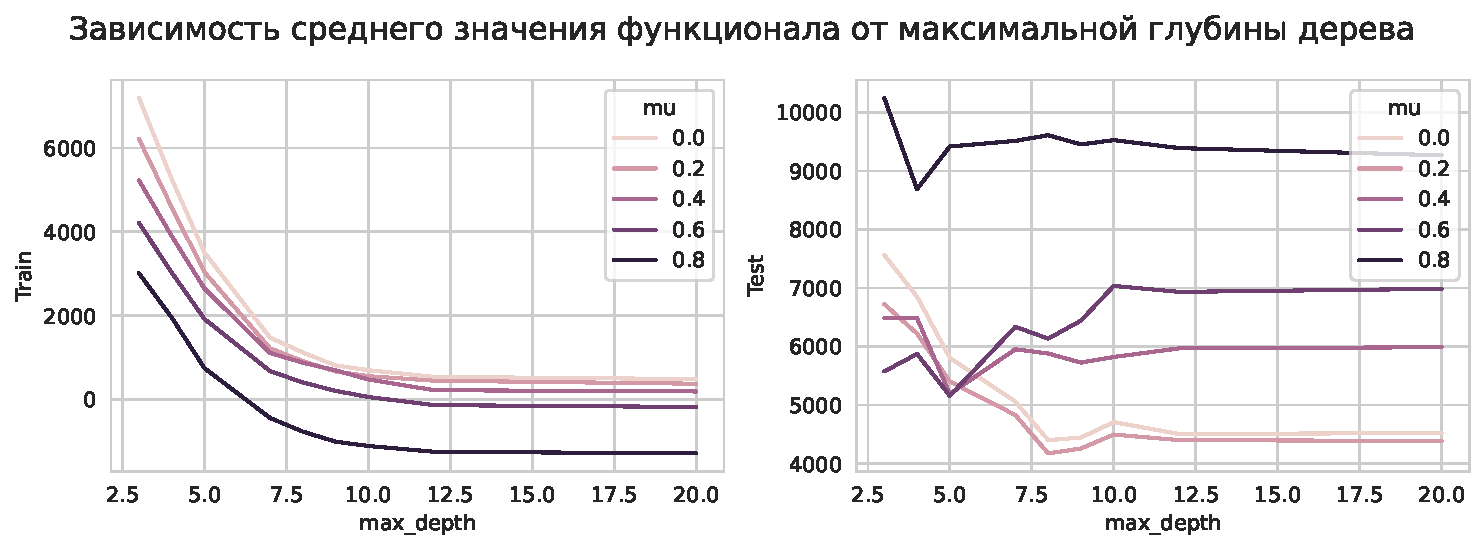
\includegraphics[width=1.0\linewidth]{../figures/max_depth_task1_gamma_08_min_2.pdf}}	
		\end{minipage}
	\end{center}
	
	\caption{График зависимости значения функционала от глубины дерева для датасета 1 при разных значениях параметра $\mu$, и при $\gamma_1 = 0.8$, $\gamma_2 = 0.2$, $min\_samples\_split = 2$. }
	\label{ris:image7}
\end{figure}

Рассмотрим поведение функционала при различных значениях параметра $\mu$ (рис. \ref{ris:image7}). Из график следует, что значение функционала на тренировочной выборке уменьшается при увеличении $\mu$, что согласуется с формулой функционала. Но противоположное наблюдается на тестовой выборке, где при увеличении параметра $\mu$ увеличиваются и значения функционала. Из этого можно сделать вывод, что сильное отдаление от ответов решающего леса ухудшает качество предсказания.


\newpage

\section{Заключение}

В данной работе исследовался метод построения дерева с помощью специального функционала, позволяющего отдаляться от уже построенного ансамбля, с целью повышения разнообразия итогового леса. Исследование производилось на данных о химических соединениях, где целевой переменной была выбрана температура плавления.
Были проведены эксперименты, показавшие корректность реализованной модели и выявившие некоторые отличия от стандартного функционала MSE.

\bibliographystyle{unsrtnat}
\bibliography{references}




\end{document}
